\chapter{Technical Analysis}
The purpose of beam steering is to increase the antenna gain in a specific direction to achieve reduction in interference and to save power. This is enabled by having the main lobe of a radiation pattern of a directional antenna pointing towards the target of transmission and reception. Beam steering is purposeful for narrow directional beams. Beam steering can be performed using manual, mechanical or electronic with the main differences being type of implementation and increasing speed of change of directivity from manual to electronic~\cite{ieee_beam_steering}~\cite{ieee_microchip_beam_steering}. This chapter explores the properties of antennas and beam steering methods, in order to understand antenna beam steering.
%https://ieeexplore-ieee-org.zorac.aub.aau.dk/document/9726284
%https://ieeexplore-ieee-org.zorac.aub.aau.dk/document/8275895

\section{Fundamentals of Antennas}
In order to develop a beam steering device for antennas it is necessary to understand antennas and their properties. Propagation, polarization, radiation characteristics are all properties of antennas that can vary based on the type of antenna.

\subsection{Propagation}
Propagation of radio waves can be described with Maxwell's equations using the polar coordinate system $\left( r, \theta, \phi, t \right)$ for antennas. In differential form, the Maxwell equations are as follows
\begin{equation}
    \begin{split}
        \nabla \times \textbf{E} & = - \frac{\partial }{\partial t} \textbf{B} \\
        \nabla \times \textbf{H} & = \textbf{J} + \frac{\partial }{\partial t} \textbf{D} \\
        \nabla \cdot \textbf{B} & = 0 \\
        \nabla \cdot \textbf{D} & = \rho
    \end{split}
\end{equation}

with \textbf{E} being the electric field with unit [\SI{}{\volt\per\meter}], \textbf{B} being induction [\SI{}{\tesla}], \textbf{H} is magnetic field [\SI{}{\ampere\per\meter}], \textbf{D} being dielectric displacement [\SI{}{\ampere\second\per\meter\squared}], \textbf{J} being the current density [\SI{}{\ampere\per\meter\squared}] and $\rho$ being electric charge density [\SI{}{\coulomb\per\meter\cubed}].

The electric field and the magnetic field are always connected; the electric field is created by the magnetic field and vice versa. The electric field and the magnetic field in polar coordinates are illustrated on figure \ref{fig:em_field} below.
\begin{figure}[h]
    \centering
    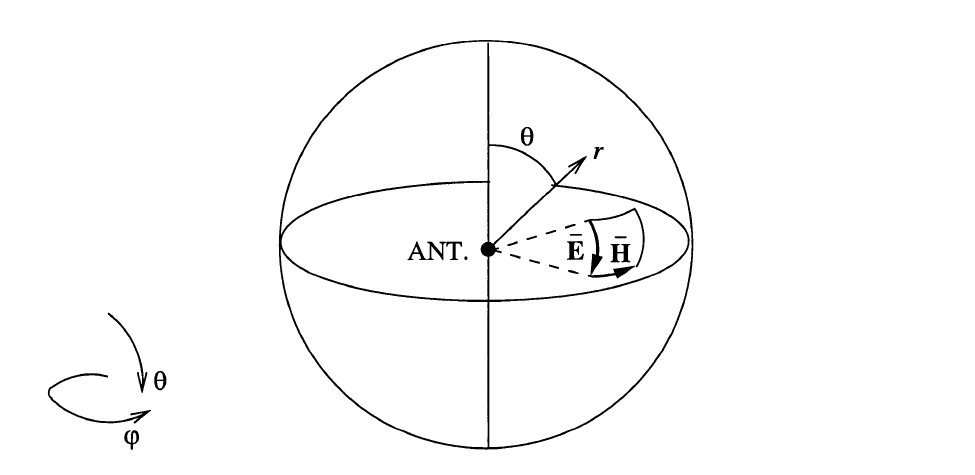
\includegraphics[width=0.6\textwidth]{figures/em_polar_coordinates.png}
    \caption{Electromagnetic field around a small antenna in far field range visualised in the polar coordinate system~\cite[p. 58]{maxwell_theory}.} \label{fig:em_field}
\end{figure}

As visualised on figure \ref{fig:em_field} the electric field only depends on the $\theta$-component and the magnetic field only on the $\phi$-component when in the far field. Assuming that $\theta$ is kept approximately constant, that the electromagnetic waves propagate in free space and that the point of observation is at a large value of $r$, the electric and magnetic fields can be approximated with the planar coordinates $\left( x, y, z, t \right)$.
\todo[inline,color=blue]{insert figure of planar coordinates and explain}

The Poynting vector describes the power density and direction of the Electromagnetic flux and is the cross product of the electric and magnetic field 
\begin{equation}
    \textbf{S} = \textbf{E} \times \textbf{H}
\end{equation}
which points in the same direction as the wave propagation. 
\todo[inline,color=blue]{add p4 rf antenna beam forming eq of power through area}
\todo[inline,color=blue]{expand maxwell eqs with frequency dependencies p4 rf antenna beam forming}

\subsubsection{Multipath propagation}
\todo[inline,color=red]{describe multipath propagation and what issues it brings and how to mitigate. Also any advantages}

\subsection{Polarization}
\todo[inline,color=red]{describe polarization and what issues it brings and how to mitigate. Also any advantages}
Different antenna designs have different radiation patterns and polarization. Table \ref{tab:antenna_types} lists a number of different antenna designs and their polarization
%https://eng.libretexts.org/Bookshelves/Electrical_Engineering/Electro-Optics/Direct_Energy_(Mitofsky)/04%3A_Antennas/4.04%3A_Antenna_Characteristics
\begin{table}
    \centering
    \begin{tabular}[h]{l|l} 
        \textbf{Type} & \textbf{Polarization} \\
        \hline
        Isotropic antenna & \\
        Dipole antenna & Linear \\
        Patch antenna & Linear, circular \\
        Horn antenna & Linear \\
        Helix antenna & Circular \\
    \end{tabular}
    \caption{Table showing polarization of some typical antenna designs.}
    \label{tab:antenna_types}
\end{table}


\subsection{Radiation Characteristics}
The radio waves are radiated to the near field and then far field free space. The far field is mathematically described as the distance $r>R_2$, with $R_2$ defined as
\begin{equation} \label{eq:far_field}
    R_2 = \frac{2 D^2}{\lambda}
\end{equation}

with $D$ being the largest dimension of the antenna or antenna array and $\lambda$ being the wavelength of the carrier frequency~\cite[p. 4]{ant_beam_form}.

The radiation characterstics of an antenna can be described by the directivity, which doesn't depend on the distance $r$ in the far field meaning that at the receiver the relation $r \gg  R_2$ is assumed. Then the directivity is
\begin{equation} \label{eq:directivity}
    D_t\left(\theta, \phi\right) = 4 \pi r^2 \frac{S_t \left(\theta, \phi\right)_{max}}{P_{t,r}}
\end{equation}

with $S_ t\left(\theta, \phi\right)_{max}$ being the maximum power density and $P_{t,r}$ being the radiated power of the antenna. The fraction $\frac{P_{t,s}}{4 \pi r^2}$ is also called the power density of the isotropic radiation of the antenna. The power of the source $P_{t,s}$ to the antenna might not equal the radiated power $P_{t,r}$ due to power loss $p_{t,l}$. Power loss can happen because of reflection loss in the input medium (typically cable), conductor loss and inductor loss. The efficiency of the antenna $\eta$ is described as the ratio of the radiated power and the sourced power %https://rfelements.com/blog/antenna-radiation-efficiency
\begin{equation} \label{eq:antenna_efficiency}
    \eta = \frac{P_{t,r}}{P_{t,s}} = \frac{P_{t,r}}{P_{t,r}+P_{t,l}}
\end{equation}

The gain $G \left( \theta, \phi \right)$ of the antenna is defined as the efficiency $\eta$ times the directivity $D$ and can be calculated as
\begin{equation} \label{eq:gain}
    G \left( \theta, \phi \right) = \eta  D\left(\theta, \phi\right) = 4 \pi r^2 \frac{S_t \left(\theta, \phi\right)_{max}}{P_{t,s}}
\end{equation}

or expressed in decibel with respect to the isotropic radiator
\begin{equation} \label{eq:gain_dbi}
    g_{dBi} = 10 \log_{10}\left(G\right)
\end{equation}

The isotropic radiator is a theoretical antenna which radiates homogeneously in all directions, meaning that the magnitude of the power density vector \textbf{S} at a distance vector \textbf{r} is constant as
\begin{equation} \label{eq:isotropic_radiation}
    \left| \frac{S \left(r, \theta, \phi \right)}{S_{max}} \right|=1
\end{equation}

It is this theoretical isotropic radiator that the gain of antennas are in respect to. The gain of a directive antenna in a certain direction is called the antenna gain $G$~\cite[pp. 10-12]{ant_beam_form}.

\subsubsection{Friis Transmission Equation}
The Friis transmission equation explains how the received power at a receiver antenna is related to the power of the transmitting antenna. The receiver antenna receives energy from the transmitting antenna and the effectiveness of this is described as the effective area $A_r\left( \theta, \phi \right)$ assuming that the antenna is placed in the origin of the polar coordinate system. If the antenna has the property of reciprocity, the effective area and the gain of the receiver antenna is related by 
\begin{equation} \label{eq:effectivate_area}
    A_r \left( \theta, \phi \right) = \frac{\lambda^2}{4 \pi} G_r \left( \theta, \phi \right)
\end{equation}

If the gain of the transmitting antenna $G_t$ is in the direction of the receiver antenna $G_r$ then the angular dependencies of the antenna properties can be surpressed. The power of the receiving antenna is equal to the power density $S_t$ multiplied by the effective area of the receiver antenna $A_r$, expressed as
\begin{equation} \label{eq:receiver_power}
    P_r = S_t A_r
\end{equation} 

As previously mentioned the directivity of an antenna does not depend on the distance $r$ from the antenna, and likewise so with the power density $S_t$, so the value of $S_t$ is equal regardless of the distance from the antenna in the far field with respects to the angular dependencies. Substituting $S_t$ and $A_r$ in equation \ref{eq:receiver_power} for $S_t$ equation isolated in \ref{eq:gain} and equation \ref{eq:effectivate_area} yields
\begin{equation} \label{eq:friis}
    \begin{split}
        P_r & = \frac{G_t P_t}{4 \pi r^2} \frac{\lambda^2 G_r}{4 \pi} \\
        & = G_t  G_r P_t \left( \frac{\lambda}{4 \pi r} \right)^2
    \end{split}
\end{equation} 

Also called Friis transmission equation~\cite[pp. 8-10]{ant_eng_hk}. $G_t$ is the gain of the transmitting antenna in the direction of the receiver and $G_r$ is the gain of the receiving antenna in the direction of the transmitter. The radiation characterstics of an antenna in the far field is called the antenna radiation pattern and will look different depending on the design of the antenna. The radiatation pattern is dependent on the anglular properties $\theta$ and $\phi$ and is usually visualised in a plane parallel to the electric field and called a \textbf{E} plane pattern or parallel to the magnetic field and called a \textbf{H} plane pattern.

\subsubsection{Antenna Design Types}

\todo[inline,color=red]{describe typical antenna designs. see p11 rf antenna beam forming}

%Because the directive antennas have areas in the radiation pattern that have very little to no gain, there are areas of the antenna radiation area that do not receive power from a transmitter. If such areas must be covered by a directive antenna, the beam of the antenna must be steered to said area. 

\section{Beam Steering Methods}

\subsection{Manual and Mechanical Steering}
\todo[inline,color=green]{explain motor control and types of motors with type of control loops}
%https://eu.aspina-group.com/en/learning-zone/columns/what-is/017/

\subsection{Electrical Steering}